\documentclass[conference]{IEEEtran}
\IEEEoverridecommandlockouts

\usepackage[utf8]{inputenc}
\usepackage[T1]{fontenc}
\usepackage[spanish]{babel}
\usepackage{icomma}          % coma decimal sin espacio en modo matematico: $0,977$
\usepackage{booktabs}
\usepackage{tabularx}
\usepackage{float}
\usepackage{cite}
\usepackage{amsmath,amssymb,amsfonts}
\usepackage{graphicx}
\usepackage{textcomp}
\usepackage{xcolor}
\usepackage{url}
\def\BibTeX{{\rm B\kern-.05em{\sc i\kern-.025em b}\kern-.08em
		T\kern-.1667em\lower.7ex\hbox{E}\kern-.125emX}}

\begin{document}
	
	\title{Técnicas de Visión por Computadora para lesiones cutáneas*\\
		{\footnotesize \textsuperscript{*}Clasificación y segmentación de imágenes aplicadas a la identificación de melanomas}}
	
	\author{\IEEEauthorblockN{1\textsuperscript{st} Civini, Tomás}
		\IEEEauthorblockA{\textit{Especialización en IA (CEIA)} \\
			\textit{Universidad de Buenos Aires}\\
			Ciudad, País \\
			tcivini@gmail.com}
		\and
		\IEEEauthorblockN{2\textsuperscript{nd} Gorosito, Pablo}
		\IEEEauthorblockA{\textit{Especialización en IA (CEIA)} \\
			\textit{Universidad de Buenos Aires}\\
			Ciudad, País \\
			Pablodgorosito@gmail.com}
		\and
		\IEEEauthorblockN{3\textsuperscript{rd} Ruggeri, Hernán}
		\IEEEauthorblockA{\textit{Especialización en IA (CEIA)} \\
			\textit{Universidad de Buenos Aires}\\
			Ciudad, País \\
			hruggeri.01@gmail.com}
		\and
		\IEEEauthorblockN{4\textsuperscript{th} Tombesi, Federico}
		\IEEEauthorblockA{\textit{Especialización en IA (CEIA)} \\
			\textit{Universidad de Buenos Aires}\\
			Comodoro Rivadavia, Argentina \\
			federicotombesi45@gmail.com}
	}
	
	\maketitle
	
	\begin{abstract}
		Se presenta un prototipo académico que clasifica imágenes dermoscópicas como benignas o malignas y segmenta la lesión con modelos preentrenados, y que detecta réplicas entre entrenamiento y prueba en la partición pública del dataset de clasificación. Se comparan EfficientNet-B0 y ResNet-18 (cabeza congelada y ajuste completo), con selección de modelo por AUC de validación y un umbral que asegura sensibilidad mínima de 0,90 en validación. La auditoría con SHA-256 no halló duplicados exactos, pero un hash perceptual encontró 6.344 pares candidatos entre particiones, agrupados en 732 grupos que obligaron a reasignar 1.209 imágenes. Con la partición corregida, ResNet-18 con ajuste completo alcanza en prueba ($n = 1.152$) un AUC de 0,977, una sensibilidad de 0,927 y una especificidad de 0,914, con 3,7 ms por imagen. La segmentación con U-Net (encoder ResNet-18) sobre ISIC 2018 alcanza un Dice de 0,883 en prueba con 9,0 ms por imagen. El sistema es un prototipo y no una herramienta diagnóstica.
	\end{abstract}
	
	\begin{IEEEkeywords}
		melanoma, clasificación de imágenes, segmentación, transfer learning, fuga de datos, U-Net.
	\end{IEEEkeywords}
	
	%====================================================================
	\section{Introducción}
	
	Este trabajo desarrolla un prototipo académico que clasifica imágenes dermoscópicas como benignas o malignas y segmenta la lesión, y muestra que la validez de sus métricas depende de la independencia entre particiones de datos. El melanoma es la forma más letal de cáncer de piel y su identificación temprana es clave para reducir la morbilidad y la mortalidad~\cite{mahmoud2024}. Como el diagnóstico se apoya en la inspección dermatoscópica por especialistas, los sistemas de deep learning se estudian como apoyo para priorizar casos sospechosos, y no como reemplazo del criterio médico.
	
	\subsection{Antecedentes recientes}
	
	Mahmoud et al.~\cite{mahmoud2024} (2024) construyen clasificadores de lesiones sobre imágenes dermoscópicas de ISIC y comparan varias arquitecturas CNN y estrategias de transfer learning con modelos preentrenados. Brutti et al.~\cite{brutti2023} (2023) comparan un método clásico de análisis de imagen con uno de deep learning sobre 25.122 imágenes dermoscópicas públicas y lo evalúan con un conjunto de prueba disjunto de 200 imágenes. Hekler et al.~\cite{hekler2024} (2024) estudian el uso de varias fotografías de una misma lesión para mejorar la clasificación de melanoma. Este proyecto sigue la línea de~\cite{mahmoud2024} y~\cite{brutti2023}, con foco en un aspecto que condiciona la validez de estos resultados: que las imágenes de prueba no tengan réplicas en el entrenamiento.
	
	\subsection{Objetivo}
	
	Diseñar y validar, con modelos preentrenados y decisiones justificadas por métricas, un prototipo que:
	\begin{itemize}
		\item clasifique imágenes dermoscópicas en benignas o malignas, y
		\item segmente la lesión.
	\end{itemize}
	El uso previsto es de apoyo y priorización, por lo que se prioriza la sensibilidad sobre la exactitud global.
	
	\subsection{Contribuciones}
	
	\begin{itemize}
		\item Comparación controlada de EfficientNet-B0 y ResNet-18, con selección de arquitectura y umbral solo con validación.
		\item Auditoría del dataset público: el hash exacto no detecta réplicas, pero un hash perceptual encuentra 6.344 pares candidatos entre particiones, que se agrupan y se reasignan.
		\item Segmentación con U-Net (encoder ResNet-18) sobre ISIC 2018 Tarea 1: Dice de 0,883 en prueba con 9,0 ms por imagen.
		\item Análisis de operación: umbral que garantiza sensibilidad mínima de 0,90 en validación y efecto de la prevalencia sobre la precisión de las alertas.
	\end{itemize}
	
	%====================================================================
	\section{Metodología}
	
	El diseño usa dos datasets públicos independientes, uno para clasificar y otro para segmentar, con particiones reproducibles (semilla 42) y selección de modelo y umbral solo con validación.
	
	\subsection{Datos}
	
	\begin{table}[H]
		\centering
		\caption{Datasets utilizados en el proyecto.}
		\label{tab:datos}
		\footnotesize
		\renewcommand{\arraystretch}{1.2}
		\begin{tabularx}{\columnwidth}{@{}p{1.5cm}>{\raggedright\arraybackslash}X>{\raggedright\arraybackslash}X@{}}
			\toprule
			\textbf{Tarea} & \textbf{Dataset} & \textbf{Contenido y partición} \\
			\midrule
			Clasificación &
			Kaggle, \emph{Melanoma skin cancer dataset: benign vs malignant}~\cite{kaggle_clasif} &
			13.879 imágenes RGB de $224\times224$ (carpetas \texttt{Benign} y \texttt{Malignant}). Prueba provista (1.000 + 1.000), reasignada tras la auditoría (Sec.~\ref{sec:auditoria}); validación: 15\,\% estratificado del entrenamiento \\
			\addlinespace
			Segmentación &
			ISIC 2018 Tarea 1~\cite{codella2019}, espejo de Kaggle~\cite{kaggle_isic}, licencia CC0 &
			2.594 pares imagen--máscara. Partición 80/10/10 al azar: 2.075 / 259 / 260 \\
			\bottomrule
		\end{tabularx}
	\end{table}
	
	Las etiquetas del dataset de clasificación provienen de los nombres de carpeta. Corresponde a la versión 1 en Kaggle; su fuente primaria y su licencia no pudieron verificarse y se declaran como limitación. Los dos datasets son distintos: el de clasificación no trae máscaras, por lo que la segmentación se entrena y evalúa por separado (Cuadro~\ref{tab:datos}).
	
	\subsection{Auditoría de integridad y partición sin réplicas}
	\label{sec:auditoria}
	
	La auditoría se hizo en dos pasos. Primero, un hash SHA-256 de cada archivo detectó 0 grupos idénticos entre particiones. Segundo, un hash perceptual dHash de 64 bits (imagen en grises de $9\times8$) con distancia de Hamming $\leq 2$ encontró 6.344 pares candidatos entre particiones. La inspección visual de una muestra de pares con distancia 0 confirmó que son la misma imagen con compresión o recortes distintos.
	
	Los pares se unieron con Union-Find en 732 grupos con más de una imagen. Cada grupo se reasignó completo a su partición mayoritaria, con desempate train $>$ val $>$ test. Esto movió 1.209 imágenes de partición. Los modelos finales se reentrenan con esta partición corregida.
	
	El agrupamiento dejó dos señales de alerta: el grupo más grande reúne 1.172 imágenes (8,4\,\% del dataset), lo que sugiere que encadenó imágenes similares sin ser réplicas, y 22 grupos contienen etiquetas contradictorias. Ambas se discuten en las limitaciones.
	
	\subsection{Clasificación}
	
	Se comparan EfficientNet-B0~\cite{tan2019} y ResNet-18~\cite{he2016}, ambas con pesos de ImageNet~\cite{russakovsky2015} y la capa final reemplazada por 2 salidas. EfficientNet-B0 partió del primer prototipo del equipo; ResNet-18 aporta una familia de redes distinta y más simple. Cada arquitectura se entrena en dos etapas con las mismas semilla, particiones y aumentos:
	
	\begin{enumerate}
		\item \textbf{Cabeza:} 8 épocas con la base congelada (incluidas las estadísticas de BatchNorm), AdamW, $\mathrm{lr} = 10^{-3}$.
		\item \textbf{Ajuste completo:} 6 épocas desde el mejor punto de la etapa 1, $\mathrm{lr} = 10^{-5}$.
	\end{enumerate}
	
	En ambas: lote de 32, entrada de $224\times224$, normalización con media y desvío de ImageNet, pérdida de entropía cruzada sin ponderar y decay de pesos $10^{-4}$. El aumento de datos (solo en entrenamiento) incluye recorte aleatorio (escala 0,85--1), giros horizontal y vertical, rotación de hasta $20^{\circ}$ y variación de brillo, contraste y saturación de 0,1. Los giros verticales son válidos porque una lesión dermatoscópica no tiene orientación natural.
	
	La arquitectura y la etapa se eligen por mayor AUC de validación. El umbral de decisión se fija también en validación: entre los que alcanzan sensibilidad $\geq 0{,}90$, el de mayor especificidad. La prueba se evalúa una sola vez con ese modelo y umbral.
	
	\subsection{Segmentación}
	
	Se entrena una U-Net~\cite{ronneberger2015} con encoder ResNet-18 preentrenado en ImageNet, usando la librería segmentation\_models\_pytorch~\cite{iakubovskii2019}. La entrada se redimensiona a $256\times256$ y las máscaras se binarizan (umbral 127) y se escalan por vecino más cercano. La pérdida combina Dice y entropía cruzada binaria (0,5 + 0,5). Se usa AdamW ($\mathrm{lr} = 10^{-4}$, decay $10^{-5}$), lote de 16 y 12 épocas; se conserva el punto con mayor Dice de validación. El aumento se aplica de forma sincronizada a imagen y máscara: giros, rotación de hasta $20^{\circ}$ y variación de brillo y contraste.
	
	\subsection{Métricas}
	
	\textbf{Clasificación:} AUC, sensibilidad, especificidad, precisión y F1 de la clase maligna, y matriz de confusión. Como la prueba está equilibrada por construcción, la precisión de las alertas se reestima para otras prevalencias con:
	\begin{equation}
		\mathrm{VPP} = \frac{\mathrm{Se}\cdot p}{\mathrm{Se}\cdot p + (1-\mathrm{Esp})(1-p)}
		\label{eq:vpp}
	\end{equation}
	donde $\mathrm{Se}$ es la sensibilidad, $\mathrm{Esp}$ la especificidad y $p$ la prevalencia supuesta.
	
	\textbf{Segmentación:} IoU y Dice por imagen, con media, mediana e intervalo de confianza del 95\,\% por bootstrap (2.000 remuestreos), más la latencia de inferencia.
	
	%====================================================================
	\section{Resultados experimentales}
	
	\subsection{Segmentación de la lesión}
	

	\begin{figure*}[!t]
		\centering
		\includegraphics[width=0.9\textwidth]{curvas_segmentacion.png}
		\caption{Segmentación: pérdida, IoU y Dice por época (entrenamiento y validación).}
		\label{fig:curvas_seg}
	\end{figure*}
	
	\begin{figure*}[!t]
		\centering
		\begin{minipage}[t]{0.48\textwidth}
			\centering
			\includegraphics[width=\linewidth]{casos_mejores.png}\\[2pt]
			{\footnotesize (a)}
		\end{minipage}\hfill
		\begin{minipage}[t]{0.48\textwidth}
			\centering
			\includegraphics[width=\linewidth]{casos_medianos.png}\\[2pt]
			{\footnotesize (b)}
		\end{minipage}\\[8pt]
		\begin{minipage}[t]{0.48\textwidth}
			\centering
			\includegraphics[width=\linewidth]{casos_peores.png}\\[2pt]
			{\footnotesize (c)}
		\end{minipage}
		\caption{Segmentación en prueba (imagen, máscara real y predicción): (a) mejores casos, (b) casos medianos y (c) peores casos.}
		\label{fig:seg2}
	\end{figure*}
	
	\begin{table}[H]
		\centering
		\caption{Segmentación en prueba ($n = 260$).}
		\label{tab:seg}
		\begin{tabular}{@{}lccc@{}}
			\toprule
			\textbf{Métrica} & \textbf{Media} & \textbf{Mediana} & \textbf{IC 95\,\% de la media} \\
			\midrule
			Dice & 0,883 & 0,932 & 0,863--0,899 \\
			IoU  & 0,813 & 0,873 & 0,791--0,832 \\
			\bottomrule
		\end{tabular}
	\end{table}
	
	La U-Net alcanza un Dice medio de 0,883 en prueba (IC 95\,\%: 0,863--0,899) con 9,0 ms por imagen, y el entrenamiento no se había estabilizado al terminar (Cuadro~\ref{tab:seg}). En validación, el Dice sube de 0,851 en la época 1 a 0,890 en la época 12, que es el punto elegido (IoU de 0,823). Según las curvas (Fig.~\ref{fig:curvas_seg}), el Dice de entrenamiento llega a cerca de 0,91 y el de validación a 0,89: la brecha es de unos 0,02 y la validación sigue subiendo al final, sin señales de sobreajuste. Por eso más épocas, mayor resolución o un encoder más grande podrían mejorar el resultado. El Dice de validación (0,890) cae dentro del intervalo de prueba.
	
	La mediana (0,932) supera a la media (0,883) por 0,050: la mayoría de las lesiones se segmenta bien, con el histograma concentrado por encima de 0,8 (Fig.~\ref{fig:hist_dice}), y pocos fallos bajan el promedio. Diez de 260 imágenes (3,8\,\%) tienen Dice menor a 0,5. El modelo tiene 14,3 M de parámetros y una latencia de 9,0 ms por imagen de $256\times256$ en la GPU de Colab con lote de una imagen, unas 110 imágenes por segundo.
	
	\begin{figure}[H]
		\centering
		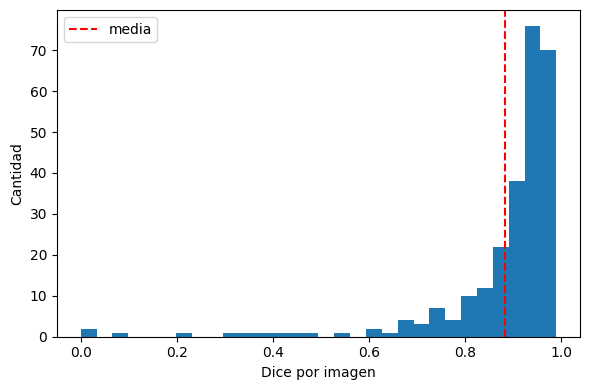
\includegraphics[width=0.95\columnwidth]{hist_dice_test.png}
		\caption{Distribución del Dice por imagen en prueba ($n = 260$); la línea roja marca la media.}
		\label{fig:hist_dice}
	\end{figure}
	
	\textbf{Peores casos.} En los cuatro peores casos de prueba (Fig.~\ref{fig:seg2}) el modelo predice una máscara vacía (Dice de 0,00 en dos imágenes) o mucho menor que la real (Dice de 0,07 y 0,21). Las lesiones tienen bajo contraste con la piel y están acompañadas de vello abundante, tinta de marcador quirúrgico o reglas del dermatoscopio. El error dominante es entonces de sub-segmentación, no de contornos inventados.
	
	La segmentación se evaluó de forma independiente: el dataset de clasificación no trae máscaras, por lo que no se midió su efecto sobre la clasificación. Además, la partición 80/10/10 es aleatoria por imagen y sin identificador de lesión, así que no se puede descartar cierta fuga entre entrenamiento y prueba.
	
	\subsection{Auditoría de datos y clasificación}
	
	La partición original del dataset de clasificación no era independiente: al agrupar las réplicas y reasignarlas, el conjunto de prueba pasa de 2.000 a 1.152 imágenes y sus casos malignos, de 1.000 a 398 (Cuadro~\ref{tab:particion}).
	
	\begin{table}[H]
		\centering
		\caption{Imágenes por partición, original y corregida.}
		\label{tab:particion}
		\begin{tabular}{@{}lrrrr@{}}
			\toprule
			& \multicolumn{2}{c}{\textbf{Original}} & \multicolumn{2}{c}{\textbf{Corregida}} \\
			\cmidrule(lr){2-3}\cmidrule(lr){4-5}
			\textbf{Partición} & Benign & Malignant & Benign & Malignant \\
			\midrule
			Entrenamiento & 5.346 & 4.751 & 5.779 & 5.417 \\
			Validación    & 943   & 839   & 756   & 775 \\
			Prueba        & 1.000 & 1.000 & 754   & 398 \\
			\bottomrule
		\end{tabular}
	\end{table}
	
	El procedimiento encontró 732 grupos de imágenes casi idénticas y movió 1.209 imágenes. Dos señales piden cautela: el grupo más grande reúne 1.172 imágenes (8,4\,\% del dataset), lo que sugiere que el agrupamiento encadenó imágenes similares sin ser réplicas, y 22 grupos contienen etiquetas contradictorias, indicio de ruido de etiquetas en el origen. Por eso la reducción de la prueba, en especial de 1.000 a 398 casos malignos, no es un conteo directo de réplicas.
	
	\textbf{Selección de modelo en validación.} ResNet-18 con ajuste completo obtuvo el mayor AUC de validación con ambas particiones y fue la arquitectura elegida (Cuadro~\ref{tab:val}).
	
	\begin{table}[H]
		\centering
		\caption{AUC de validación por modelo y etapa.}
		\label{tab:val}
		\begin{tabular}{@{}llcc@{}}
			\toprule
			\textbf{Modelo} & \textbf{Etapa} & \textbf{Original} & \textbf{Corregida} \\
			\midrule
			EfficientNet-B0 & Cabeza          & 0,952 & 0,944 \\
			EfficientNet-B0 & Ajuste completo & 0,951 & 0,941 \\
			ResNet-18       & Cabeza          & 0,946 & 0,937 \\
			ResNet-18       & Ajuste completo & 0,960 & 0,957 \\
			\bottomrule
		\end{tabular}
	\end{table}
	
	\textbf{Costo computacional} (lote de una imagen, GPU de Colab; Cuadro~\ref{tab:costo}).
	
	\begin{table}[H]
		\centering
		\caption{Costo computacional.}
		\label{tab:costo}
		\begin{tabular}{@{}lcc@{}}
			\toprule
			\textbf{Modelo} & \textbf{Parámetros (M)} & \textbf{Latencia (ms)} \\
			\midrule
			EfficientNet-B0 & 4,01  & 7,5 \\
			ResNet-18       & 11,18 & 3,7 \\
			\bottomrule
		\end{tabular}
	\end{table}
	
	ResNet-18 tiene 2,8 veces más parámetros que EfficientNet-B0 y aun así la mitad de latencia: tener menos parámetros no implica mayor velocidad.
	
	\textbf{Evaluación en prueba.} La columna original se conserva solo como referencia; la corregida es el resultado que se reporta, con intervalos de confianza del 95\,\% por bootstrap (2.000 remuestreos) (Cuadro~\ref{tab:test}).
	
	\begin{table}[H]
		\centering
		\caption{Prueba con ResNet-18 ajustada.}
		\label{tab:test}
		\footnotesize
		\begin{tabular}{@{}lcc@{}}
			\toprule
			\textbf{Métrica} & \textbf{Original} & \textbf{Corregida} \\
			& ($n = 2.000$) & ($n = 1.152$) \\
			\midrule
			Umbral (validación)   & 0,413   & 0,576 \\
			AUC                   & 0,974   & 0,977 (0,969--0,984) \\
			Sensibilidad          & 0,901   & 0,927 (0,902--0,951) \\
			Especificidad         & 0,924   & 0,914 (0,892--0,934) \\
			F1 (maligna)          & 0,911   & 0,887 \\
			Falsos neg.\ / pos.   & 99 / 76 & 29 / 65 \\
			\bottomrule
		\end{tabular}
	\end{table}
	
	Con la partición corregida, el umbral elegido en validación (0,576) logró una sensibilidad de 0,927 en prueba, frente a 0,940 con el umbral 0,5; la especificidad subió de 0,893 a 0,914. Hay 29 falsos negativos y 65 falsos positivos, contra 24 y 81 con 0,5: el umbral mayor cambia 5 falsos negativos más por 16 falsos positivos menos. Con esa sensibilidad y especificidad, y una prevalencia supuesta de 5\,\%, solo el 36,1\,\% de las alertas serían lesiones malignas (54,4\,\% con 10\,\%), según la ecuación~(\ref{eq:vpp}). Es un cálculo ilustrativo, no una medición clínica.
	
	\textbf{Efecto de la fuga.} El AUC de prueba pasó de 0,974 a 0,977: no cae al corregir la partición. Como las pruebas son distintas (2.000 imágenes con 50\,\% de malignas frente a 1.152 con 35\,\%) y el agrupamiento pudo encadenar imágenes que no eran réplicas, estos números no permiten aislar ni descartar un efecto de la fuga. La F1 y la precisión no son comparables entre columnas porque dependen de la prevalencia. Con 398 casos malignos, los intervalos son más anchos que los de una prueba de 1.000.
	
	La prueba corregida conserva imágenes de la prueba original, que ya se había usado para evaluar una primera versión del modelo durante el desarrollo; por eso no es una medición estrictamente independiente.
	
	%====================================================================
	\section{Conclusiones}
	
	Todas las conclusiones se apoyan en la partición corregida y en una única evaluación sobre la prueba.
	
	\begin{enumerate}
		\item \textbf{Auditoría.} Un hash exacto no alcanza para auditar un dataset dermoscópico público: SHA-256 encontró 0 duplicados entre particiones y dHash encontró 6.344 pares candidatos, agrupables en 732 grupos que obligaron a mover 1.209 imágenes. Las particiones deben construirse por grupos de réplicas.
		\item \textbf{Segmentación.} La U-Net con encoder ResNet-18 alcanza un Dice de 0,883 (IC 95\,\%: 0,863--0,899) y un IoU de 0,813 en prueba ($n = 260$), con 9,0 ms por imagen, lo que permite uso interactivo.
		\item \textbf{Errores de segmentación.} El 3,8\,\% de las imágenes tiene Dice menor a 0,5 y la mediana (0,932) supera a la media (0,883): los errores se concentran en pocos casos difíciles, de bajo contraste, con vello, tinta o reglas, donde el modelo sub-segmenta o predice una máscara vacía.
		\item \textbf{Arquitectura.} ResNet-18 con ajuste completo obtuvo el mayor AUC de validación (0,957 frente a 0,944 de EfficientNet-B0). El ajuste completo mejoró a ResNet-18 (0,937 a 0,957) y no a EfficientNet-B0 (0,944 a 0,941). ResNet-18 tiene 2,8 veces más parámetros pero la mitad de latencia (3,7 frente a 7,5 ms).
		\item \textbf{Desempeño en prueba.} Con la partición corregida ($n = 1.152$), el modelo alcanza un AUC de 0,977 (0,969--0,984), sensibilidad de 0,927 (0,902--0,951) y especificidad de 0,914 (0,892--0,934), con 29 falsos negativos y 65 falsos positivos.
		\item \textbf{Umbral de operación.} Fijar en validación una sensibilidad mínima de 0,90 dio un umbral de 0,576 y se trasladó a prueba (0,927). Frente al umbral 0,5 cambia 5 falsos negativos más por 16 falsos positivos menos: la sensibilidad es una decisión de diseño explícita.
		\item \textbf{Prevalencia.} Con una prevalencia supuesta de 5\,\%, solo el 36,1\,\% de las alertas serían malignas (54,4\,\% con 10\,\%), aunque la prueba equilibrada muestre alta precisión; por eso se reportan sensibilidad, especificidad y AUC.
		\item \textbf{Efecto de la fuga.} El AUC de prueba pasó de 0,974 a 0,977 al corregir la partición, por lo que el efecto de la fuga no puede aislarse con estos datos: las pruebas difieren en tamaño y prevalencia, y el agrupamiento pudo encadenar imágenes no replicadas.
	\end{enumerate}
	
	\subsection*{Limitaciones y trabajo futuro}
	\begin{itemize}
		\item El grupo más grande reúne 1.172 imágenes y 22 grupos tienen etiquetas contradictorias. Un análisis de sensibilidad con distancia de Hamming 0 (réplicas casi seguras) permitiría separar réplicas reales de encadenamiento.
		\item Ningún dataset trae identificadores de paciente o lesión, por lo que no se garantiza independencia por paciente.
		\item La fuente primaria, la versión y la licencia del dataset de clasificación no pudieron verificarse.
		\item La prueba corregida conserva imágenes de la prueba original usada durante el desarrollo; una medición estrictamente nueva requiere un conjunto externo con origen y etiquetas verificables.
		\item La segmentación y la clasificación son modelos independientes sobre datasets distintos. El siguiente paso es segmentar, recortar y clasificar, y medir si eso mejora la sensibilidad.
		\item El sistema es un prototipo académico: no tiene validación clínica y sus puntajes no son probabilidades calibradas.
	\end{itemize}
	
	%====================================================================
	% Orden = orden de primera cita en el texto (numeracion IEEE).
	\begin{thebibliography}{00}
		
		\bibitem{mahmoud2024}
		H.~Mahmoud, O.~A. Omer, S.~Ragab, H.~Esmaiel y M.~Abdel-Nasser, ``Classifying melanoma in ISIC dermoscopic images using efficient convolutional neural networks and deep transfer learning,'' \textit{Traitement du Signal}, vol.~41, no.~2, pp.~679--691, 2024, doi: 10.18280/ts.410211.
		
		\bibitem{brutti2023}
		F.~Brutti, F.~La Rosa, L.~Lazzeri, C.~Benvenuti, G.~Bagnoni, D.~Massi y M.~Laurino, ``Artificial intelligence algorithms for benign vs.\ malignant dermoscopic skin lesion image classification,'' \textit{Bioengineering}, vol.~10, no.~11, p.~1322, 2023, doi: 10.3390/bioengineering10111322.
		
		\bibitem{hekler2024}
		% TODO: completar volumen, numero y paginas antes de entregar.
		A.~Hekler \textit{et al.}, ``Using multiple real-world dermoscopic photographs of one lesion improves melanoma classification via deep learning,'' \textit{J. Am. Acad. Dermatol.}, 2024.
		
		\bibitem{kaggle_clasif}
		ailearner-researchlab, ``Melanoma skin cancer dataset: benign vs malignant,'' Kaggle. [En línea]. Disponible: \url{https://www.kaggle.com/datasets/ailearner-researchlab/melanoma-skin-cancer-dataset-benign-vs-malignant}
		
		\bibitem{codella2019}
		N.~Codella \textit{et al.}, ``Skin lesion analysis toward melanoma detection 2018: A challenge hosted by the International Skin Imaging Collaboration (ISIC),'' arXiv:1902.03368, 2019.
		
		\bibitem{kaggle_isic}
		tschandl (usuario de Kaggle), ``ISIC2018 Challenge Task1 Data (Segmentation),'' Kaggle, espejo del desafío ISIC 2018. [En línea]. Disponible: \url{https://www.kaggle.com/datasets/tschandl/isic2018-challenge-task1-data-segmentation}
		
		\bibitem{tan2019}
		M.~Tan y Q.~V. Le, ``EfficientNet: Rethinking model scaling for convolutional neural networks,'' en \textit{Proc. ICML}, 2019, pp.~6105--6114.
		
		\bibitem{he2016}
		K.~He, X.~Zhang, S.~Ren y J.~Sun, ``Deep residual learning for image recognition,'' en \textit{Proc. IEEE CVPR}, 2016, pp.~770--778.
		
		\bibitem{russakovsky2015}
		O.~Russakovsky \textit{et al.}, ``ImageNet large scale visual recognition challenge,'' \textit{Int. J. Comput. Vis.}, vol.~115, no.~3, pp.~211--252, 2015.
		
		\bibitem{ronneberger2015}
		O.~Ronneberger, P.~Fischer y T.~Brox, ``U-Net: Convolutional networks for biomedical image segmentation,'' en \textit{Proc. MICCAI}, 2015, pp.~234--241.
		
		\bibitem{iakubovskii2019}
		P.~Iakubovskii, ``Segmentation Models Pytorch,'' GitHub, 2019. [En línea]. Disponible: \url{https://github.com/qubvel/segmentation_models.pytorch}
		
	\end{thebibliography}
	
\end{document}